\documentclass[12pt]{article}
\usepackage{latexsym, amssymb, amsmath, amsfonts, amscd, amsthm, xcolor, pgfplots}
\usepackage{framed}
\usepackage[margin=1in]{geometry}
\linespread{1} %Change the line spacing only if instructed to do so.
\pgfplotsset{compat=1.14}
\newenvironment{problem}[2][Problem]
{
	\begin{trivlist} 
		\item[\hskip \labelsep {\bfseries #1 #2:}]
	}
{
	\end{trivlist}
	}

\newenvironment{solution}[1][Solution]
{
	\begin{trivlist} 
		\item[\hskip \labelsep {\itshape #1:}]
	}
	{
	\end{trivlist}
}

\newenvironment{collaborators}[5][Collaborator(s)]
{
	\begin{trivlist} 
		\item[\hskip \labelsep {\bfseries #2:}]
	}
	{
	\end{trivlist}
}

%%%%%%%%%%%%%%%%%%%%%%%%%%%%%%%%%%%%%%%%%%%%%%%%%%
%%%%%%%%%%%%%%%%%%%%%%%%%%%%%%%%%%%%%%%%%%%%%%%%%%
%%%%%%%%%%%%%%%%%%%%%%%%%%%%%%%%%%%%%%%%%%%%%%%%%%
%
%
%    You need only modify code below this block.
%
%
%%%%%%%%%%%%%%%%%%%%%%%%%%%%%%%%%%%%%%%%%%%%%%%%%%
%%%%%%%%%%%%%%%%%%%%%%%%%%%%%%%%%%%%%%%%%%%%%%%%%%
%%%%%%%%%%%%%%%%%%%%%%%%%%%%%%%%%%%%%%%%%%%%%%%%%%
%
\title{Numerical simulation of a Coupled Double Pendulum Oscillator} %Change this to the assignment you are submitting.
\author{Oleksandr Yardas, Sage Kaplan-Goland, and Russell Wang} %Change this to your name.
\date{Due Date: 00/00/2018 } %Change this to the due date for the assignment you are submitting.
\begin{document}
	\maketitle
	\thispagestyle{empty}
	
	\newpage
	\begin{figure}
	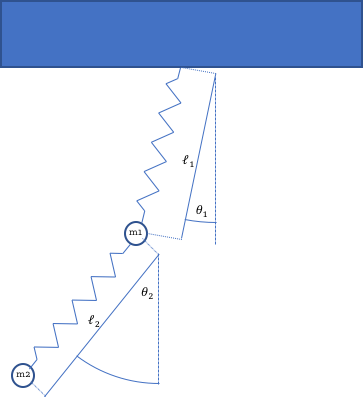
\includegraphics[width=250pt]{figure1.png}
	\caption{Coupled oscillator double pendulum.}
	\label{fig:figure1}
	\end{figure}
\begin{problem}{1}
We constructed a Lagrangian for this system:
\begin{align*}
\mathcal{L}=&\mathcal{T}-\mathcal{V}\\
\mathcal{T}=&\frac{1}{2} m_1 v_1 ^2 + \frac{1}{2} m_2 v_2 ^2 \\
\mathcal{V}=&m_1 g y_1 + m_2 g y_2 +\frac{1}{2} k_1 (l_1 -l_{0_1})^2 + \frac{1}{2} k_2  (l_2-l_{0_2}) ^2\\
l_1=& l_{1_0} + \Delta l_1 (t)\\
l_2=& l_{2_0} + \Delta l_2 (t) \\
y_1 =& -l_1 \cos (\theta_1)\\
y_2 =& -l_1 \cos(\theta_1) - l_2 \cos (\theta_2)\\
v_1 ^2 =& \dot{l}_1 ^2 + l_1 ^2 \dot{\theta} _1 ^2\\
v_2 ^2 =&  \dot{l}_1 ^2 + l_1 ^2 \dot{\theta} _1 ^2 +  \dot{l}_2 ^2 + l_2 ^2 \dot{\theta} _2 ^2 + 2 \sin (\theta_1 - \theta_2) \cdot(\dot{l}_1 l_2 \dot{\theta}_2 - \dot{l}_2 l_1 \dot{\theta}_1) + 2\cos (\theta_1 - \theta_2) \cdot (\dot{l}_1 \dot{l}_2 + l_1\dot{\theta}_1 l_2 \dot{\theta}_2)
\end{align*}
So we get
\begin{align*}
\mathcal{L} (t, l_1, \dot{l}_1, \theta_1, \dot{\theta}_1, l_2, \dot{l}_2, \theta_2, \dot{\theta}_2)=& \frac{1}{2} m_1 (\dot{l}_1 ^2 + l_1 ^2 \dot{\theta} _1 ^2) + \frac{1}{2} m_2 (\dot{l}_1 ^2 + l_1 ^2 \dot{\theta} _1 ^2 +  \dot{l}_2 ^2 + l_2 ^2 \dot{\theta} _2 ^2\\
+&2 \sin (\theta_1 - \theta_2) \cdot(\dot{l}_1 l_2 \dot{\theta}_2 - \dot{l}_2 l_1 \dot{\theta}_1) + 2\cos (\theta_1 - \theta_2) \cdot (\dot{l}_1 \dot{l}_2 + l_1\dot{\theta}_1 l_2 \dot{\theta}_2))\\
+&m_1 g l_1 \cos (\theta_1) +m_2 g (l_1 \cos(\theta_1) + l_2 \cos (\theta_2)) -\frac{1}{2} k_1 (l_1 -l_{0_1})^2 - \frac{1}{2} k_2  (l_2 -l_{0_2})^2
\end{align*}
We then solved the Lagrangian for each variable, obtaining four coupled equations:
%\begin{align*}
%
%\ddot{\theta}_1 =&( g m_1 l_1 \sin(\theta_1) + g m_2 l_1 \sin(\theta_1) + 2 m_1 l_1 \dot{l}_1 \dot{\theta}_1 + 2 m_2 l_1 \dot{l}_1 \dot{\theta}_1 + 2 m_2 \cos(\theta_1 - \theta_2) l_1 \dot{l}_2 \dot{\theta}_2\\
%+& m_2 l_1 l_2 \sin(\theta_1 - \theta_2) \dot{\theta}_2 ^2 - m_2 l_1 \sin(\theta_1 - \theta_2) \ddot{l}_2 + m_2 \cos (\theta_1 - \theta_2) l_1 l_2 \ddot{\theta}_2) \frac{1}{-m_1 l_1 ^2 - m_2 l_1 ^2}\\
%
%
%
%\ddot{l}_1=& \frac{1}{-m_1 -m_2} ( -g m_1\cos(\theta_1) - g m_2 \cos(\theta_1) + k_1 l_1 - m_1 l_1 \dot{\theta}_1 ^2 - m_2  l_1\dot{\theta}_1 ^2 + 2 m_2 \sin(\theta_1 - \theta_2) \dot{l}_2 \dot{\theta}_2\\
%-& m_2 \cos(\theta_1 -\theta_2) l_2 \dot{\theta}_2 ^2 + m_2 \cos(\theta_1 - \theta_2) \ddot{l}_2 + m_2 l_2 \sin(\theta_1-\theta_2)\ddot{\theta}_2)\\
%
%
%
%\ddot{\theta}_2 =& -\frac{1}{m_2 l_2 ^2}(g m_2 l_2 \sin(\theta_2) + 2 m_2 \cos(\theta_1 - \theta_2) l_2 \dot{l}_1 \dot{\theta}_1 - m_2 l_1 l_2 \sin(\theta_1 - \theta_2) \dot{\theta}_1 ^2 + 2 m_2 l_2 \dot{l}_2 \dot{\theta}_2\\
%+& m_2 l_2 \sin(\theta_1 - \theta_2) \ddot{l}_1 + m_2 \cos(\theta_1 - \theta_2) l_1 l_2 \ddot{\theta}_1)\\
%
%
%
%\ddot{l}_2 =& -\frac{1}{m_2}(-g m_2 \cos(\theta_2) + k_2 l_2 - 2 m_2 \sin(\theta_1 - \theta_2) \dot{l}_1 \dot{\theta}_1 - m_2 \cos(\theta_1 - \theta_2) l_1 \dot{\theta}_1 ^2 - m_2 l_2 \dot{\theta}_2 ^2 \\
%+& m_2 \cos(\theta_1 - \theta_2) \ddot{l}_1 - m_2 l_1 \sin(\theta_1 - \theta_2) \ddot{\theta}_1)\\
%\end{align*}
%These seem unwieldy at first, but it turns out that we can collect terms to get something where the symmetry is apparent:
\begin{align*}
\ddot{\theta}_1=&\frac{(m_1  + m_2) (g \sin(\theta_1) + 2 \dot{l}_1 \dot{\theta}_1) + m_2((2 \dot{l}_2 \dot{\theta}_2 + l_2 \ddot{\theta}_2) \cos(\theta_1 - \theta_2) + (l_2 \dot{\theta}_2 ^2  -  \ddot{l}_2)\sin(\theta_1 - \theta_2))}{-(m_1 + m_2) l_1}\\
%
\ddot{l}_1=& \frac{(-m_1 - m_2) (g\cos(\theta_1) + l_1 \dot{\theta}_1 ^2) + k_1 (l_1-l_{0_1}) + m_2 ((2  \dot{l}_2 \dot{\theta}_2 + l_2 \ddot{\theta}_2)\sin(\theta_1 - \theta_2) +(\ddot{l}_2 - l_2 \dot{\theta}_2 ^2)\cos(\theta_1 -\theta_2))}{-(m_1 +m_2)}\\
%
\ddot{\theta}_2 =&\frac{g\sin(\theta_2) + 2\dot{l}_2 \dot{\theta}_2 + (2 \dot{l}_1 \dot{\theta}_1 +  l_1 \ddot{\theta}_1)\cos(\theta_1 - \theta_2) + (\ddot{l}_1 - l_1 \dot{\theta}_1 ^2)\sin(\theta_1 - \theta_2)}{-l_2}\\
%
\ddot{l}_2 =&g \cos(\theta_2) + l_2 \dot{\theta}_2 ^2  -\frac{k_2}{m_2}(l_2 - l_{0_2})  + ((2 \dot{l}_1 \dot{\theta}_1 + l_1 \ddot{\theta}_1 )\sin(\theta_1 - \theta_2) + ( l_1 \dot{\theta}_1 ^2 - \ddot{l}_1)\cos(\theta_1 - \theta_2))
\end{align*}
This system can be solved (with the assistance of Mathematica) to give unique solutions for $\ddot{\theta}_1, \ddot{l}_1, \ddot{\theta}_2,\ddot{l}_2$:
\begin{align*}
\ddot{\theta}_1 =&\frac{-g m_1 \sin(\theta_1) - k_2 (l_2-l_{0_2}) \sin(\theta_1 - \theta_2) - 2 m_1 \dot{l}_1 \dot{\theta}_1}{m_1 l_1}\\
%
\ddot{l}_1 =& \frac{g m_1 \cos(\theta_1) - k_1(l_1- l_{0_1}) +k_2 (l_2-l_{0_2}) \cos(\theta_1 - \theta_2) + l_1 m_1 \dot{\theta}_1 ^2}{m_1}\\
%
\ddot{\theta}_2 =& \frac{k_1 (l_1-l_{0_1}) \sin(\theta_1 -\theta_2) - 2 m_1 \dot{l}_2 \dot{\theta}_2}{m_1 l_2}\\
%
\ddot{l}_2 =& \frac{k_1 m_2 (l_1-l_{0_1}) \cos(\theta_1 - \theta_2) -k_2(l_2 - l_{0_2}) (m_1+m_2) + l_2 m_1 m_2 \dot{\theta}_2 ^2}{m_1 m_2}\\
\end{align*}
Which further reduce to:
\begin{align*}
\ddot{\theta}_1 =& -\frac{g}{l_1} \sin(\theta_1) - \frac{k_2}{m_1} \cdot \frac{l_2-l_{0_2}}{l_1} \sin(\theta_1 - \theta_2) - 2 \dot{\theta}_1 \frac{\dot{l}_1}{l_1}\\
%
\ddot{l}_1 =& g \cos(\theta_1) - \frac{k_1}{m_1}(l_1- l_{0_1}) + \frac{k_2}{m_1} (l_2-l_{0_2}) \cos(\theta_1 - \theta_2) + l_1 \dot{\theta}_1 ^2\\
%
\ddot{\theta}_2 =& \frac{k_1}{m_1}\cdot \frac{l_1-l_{0_1}}{l_2} \sin(\theta_1 -\theta_2) - 2 \frac{\dot{l}_2 \dot{\theta}_2}{l_2}\\
%
\ddot{l}_2 =& \frac{k_1}{m_1} (l_1-l_{0_1}) \cos(\theta_1 - \theta_2) -(\frac{k_2}{m_2} +\frac{k_2}{m_1})(l_2 - l_{0_2}) + l_2 \dot{\theta}_2 ^2\\
\end{align*}
If we add damping and air resistance, we get
\begin{align*}
\ddot{\theta}_1 =& -\frac{g}{l_1} \sin(\theta_1) - \frac{k_2}{m_1} \cdot \frac{l_2-l_{0_2}}{l_1} \sin(\theta_1 - \theta_2) - 2 \dot{\theta}_1 \frac{\dot{l}_1}{l_1} - \beta_1 \dot{\theta}_1\\
%
\ddot{l}_1 =& g \cos(\theta_1) - \frac{k_1}{m_1}(l_1- l_{0_1}) + \frac{k_2}{m_1} (l_2-l_{0_2}) \cos(\theta_1 - \theta_2) + l_1 \dot{\theta}_1 ^2 - \gamma_1 \dot{l}_1\\
%
\ddot{\theta}_2 =& \frac{k_1}{m_1}\cdot \frac{l_1-l_{0_1}}{l_2} \sin(\theta_1 -\theta_2) - 2 \dot{\theta}_2 \frac{\dot{l}_2}{l_2} - \beta_2 \dot{\theta}_2\\
%
\ddot{l}_2 =& \frac{k_1}{m_1} (l_1-l_{0_1}) \cos(\theta_1 - \theta_2) -(\frac{k_2}{m_2} +\frac{k_2}{m_1})(l_2 - l_{0_2}) + l_2 \dot{\theta}_2 ^2 - \gamma_2 \dot{l}_2\\
\end{align*}
We can also approximate small $\theta_1,\theta_2$ in the Lagrangian:
\begin{align*}
\mathcal{L} (t, l_1, \dot{l}_1, \theta_1, \dot{\theta}_1, l_2, \dot{l}_2, \theta_2, \dot{\theta}_2)=& \frac{1}{2} m_1 (\dot{l}_1 ^2 + l_1 ^2 \dot{\theta} _1 ^2) + \frac{1}{2} m_2 (\dot{l}_1 ^2 + l_1 ^2 \dot{\theta} _1 ^2 +  \dot{l}_2 ^2 + l_2 ^2 \dot{\theta} _2 ^2\\
+&2 (\theta_1 - \theta_2) \cdot(\dot{l}_1 l_2 \dot{\theta}_2 - \dot{l}_2 l_1 \dot{\theta}_1) + 2(1-\frac{(\theta_1 - \theta_2)^2}{2}) \cdot (\dot{l}_1 \dot{l}_2 + l_1\dot{\theta}_1 l_2 \dot{\theta}_2))\\
+&m_1 g l_1 (1-\frac{\theta_1 ^2}{2}) +m_2 g (l_1 (1-\frac{\theta_1 ^2}{2}) + l_2 (1-\frac{\theta_2 ^2}{2})) -\frac{1}{2} k_1 (l_1 -l_{0_1})^2 - \frac{1}{2} k_2  (l_2 -l_{0_2})^2
\end{align*}
giving us
\begin{align*}
\ddot{\theta}_1 =& (m_2 l_2 (\theta_1 - \theta_2)\dot{l}_1 \dot{l}_2 + m_2 l_1 ^2 l_2 (\theta_1 - \theta_2) \dot{\theta}_1 ^2 - l_1 k_2 l_2 ^2 (\theta_1 - \theta_2) + l_1 m_2 (\theta_1 - \theta_2) \dot{l}_1 \dot{l}_2\\
+& l_1 l_2  k_2 l_{2_0} \theta_1 - l_1 l_2 g m_1 \theta_1 - l_1  l_2  k_2 l_{2_0} \theta_2 + l_1 l_2  \frac{1}{2} g m_2 \theta_2 (\theta_1- \theta_2)^2 - l_1 l_2  \frac{1}{2} g m_2 \theta_1 ^2 \theta_2 - l_1 l_2  \dot{l}_1 \dot{\theta}_1 2 m_1 + l_1 l_2  \dot{l}_1 \dot{\theta}_1 m_2 (\theta_1-\theta_2)^2\\
+& m_2 l_2 (\theta_1 - \theta_2)^2 \dot{l}_1 \dot{\theta}_2 + m_2 l_2 ^2 (\theta_1 - \theta_2) \dot{\theta}_2 ^2) \cdot (l_1 ^2 l_2 (m_1 - m_2 (\theta_1 - \theta_2)^2))^{-1}\\
%
\ddot{l}_1 =& g \cos(\theta_1) - \frac{k_1}{m_1}(l_1- l_{0_1}) + \frac{k_2}{m_1} (l_2-l_{0_2}) \cos(\theta_1 - \theta_2) + l_1 \dot{\theta}_1 ^2\\
%
\ddot{\theta}_2 =& \frac{k_1}{m_1}\cdot \frac{l_1-l_{0_1}}{l_2} \sin(\theta_1 -\theta_2) - 2 \frac{\dot{l}_2 \dot{\theta}_2}{l_2}\\
%
\ddot{l}_2 =& \frac{k_1}{m_1} (l_1-l_{0_1}) \cos(\theta_1 - \theta_2) -(\frac{k_2}{m_2} +\frac{k_2}{m_1})(l_2 - l_{0_2}) + l_2 \dot{\theta}_2 ^2\\
\end{align*}

\end{problem}


\end{document}